%auto-ignore
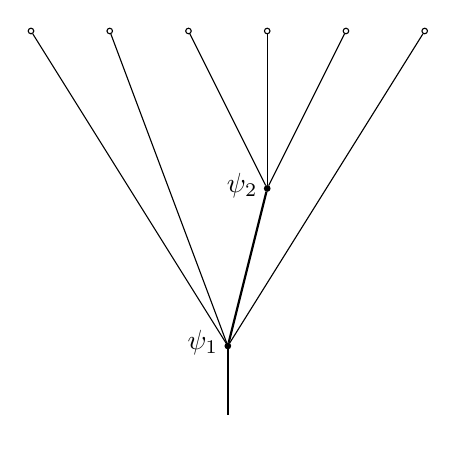
\begin{tikzpicture}
\tikzset{point/.style = {draw, circle, fill=black, minimum size=2pt,inner sep=0pt}}
\def\len{2};
\node[point,label={[left]:$\psi_1$}] (I) at (0,0) {};
\node[point,label={[left]:$\psi_2$}] (II) at (0.5,\len) {};
\node (III) at (0,-.5*\len) {};
\node[point, style={fill=white}] (v1) at (-2.5,2*\len) {};
\node[point, style={fill=white}] (v2) at (-1.5,2*\len) {};
\node[point, style={fill=white}] (v3) at (-.5,2*\len) {};
\node[point, style={fill=white}] (v4) at (.5,2*\len) {};
\node[point, style={fill=white}] (v5) at (1.5,2*\len) {};
\node[point, style={fill=white}] (v6) at (2.5,2*\len) {};
\draw[thick] (I) to (II);
\draw[thick] (I) to (III);
\draw[thin] (I) to (v1);
\draw[thin] (I) to (v2);
\draw[thin] (II) to (v3);
\draw[thin] (II) to (v4);
\draw[thin] (II) to (v5);
\draw[thin] (I) to (v6);
\end{tikzpicture}